% Created 2020-09-22 Tue 17:03
% Intended LaTeX compiler: lualatex
\documentclass[11pt]{article}
\usepackage{graphicx}
\usepackage{grffile}
\usepackage{longtable}
\usepackage{wrapfig}
\usepackage{rotating}
\usepackage[normalem]{ulem}
\usepackage{amsmath}
\usepackage{textcomp}
\usepackage{amssymb}
\usepackage{capt-of}
\usepackage{hyperref}
\usepackage{tabularx}
\usepackage{etoolbox}
\makeatletter
\def\dontdofcolorbox{\renewcommand\fcolorbox[4][]{##4}}
\AtBeginEnvironment{minted}{\dontdofcolorbox}
\makeatother
\usepackage[newfloat]{minted}
\author{Mark Armstrong}
\date{September 11th, 2020}
\title{Computer Science 3MI3 – 2020 homework 1\\\medskip
\large Implementing trees in Scala}
\hypersetup{
   pdfauthor={Mark Armstrong},
   pdftitle={Computer Science 3MI3 – 2020 homework 1},
   pdfkeywords={},
   pdfsubject={Introductory homework on Scala and trees},
   pdfcreator={Emacs 27.0.90 (Org mode 9.3.8)},
   pdflang={English},
   colorlinks,
   linkcolor=blue,
   citecolor=blue,
   urlcolor=blue
   }
\begin{document}

\maketitle
\tableofcontents


\section*{Introduction}
\label{sec:org1d70e2e}
Scala is a purely object-oriented language on the JVM,
and in addition to object-oriented abstractions
it fully supports the abstractions of \emph{functional programming}.
We are interested in it because of this functional programming support.

Herein we implement several types of trees,
the de facto example of an \emph{algebraic datatype},
along with \texttt{flatten}-ing functions
which convert those trees to the less structured type of lists.

\section*{Boilerplate}
\label{sec:orgc97567e}
\subsection*{Submission procedures}
\label{sec:orgad7dc07}
\subsubsection*{Submission method}
\label{sec:org7d085d9}

Homework should be submitted to your McMaster CAS Gitlab respository
in the \texttt{cs3mi3-fall2020} project.

Ensure that you have \textbf{pushed} the commits to the remote repository
in time for the deadline, and not just committed to your local copy.

\subsubsection*{Naming requirements}
\label{sec:orgdfebb9f}

Place all files for the homework
inside a folder titled \texttt{hn}, where \texttt{n} is the number of the homework.
So, for homework 1, the use the folder \texttt{h1}, for homework 2 the folder \texttt{h2}, etc.
Ensure you do not capitalise the \texttt{h}.

Unless otherwise instructed in the homework questions,
place all of your code for the homework
in a single file in the \texttt{hn} folder named \texttt{hn.ext},
where \texttt{ext} is the appropriate extension for the language used
according to this list:
\begin{itemize}
\item For Scala, \texttt{ext} is \texttt{sc}.
\item For Prolog, \texttt{ext} is \texttt{pl}.
\item For Ruby, \texttt{ext} is \texttt{rb}.
\item For Clojure, \texttt{ext} is \texttt{clg}.
\end{itemize}
If multiple languages are used in the homework,
submit a \texttt{hn.ext} file for each language.

\begin{center}
\textbf{If the language supports multiple different file extensions,}
\textbf{you must still follow the extension conventions above.}
\end{center}

\begin{center}
\textbf{Incorrect naming of files may result in up to a 10\% deduction in your grade.}
\end{center}

\subsubsection*{Do not submit testing or diagnostic code}
\label{sec:org52cd497}

Unless you are instructed to do so in the homework questions,
\textbf{you should not submit testing code with your homework submission}.

This includes
\begin{itemize}
\item any \texttt{main} function,
\item any \texttt{print} statements which output information
\textbf{that is not directly requested as console output}
\textbf{in the homework questions}.
\end{itemize}

If you do not wish to remove diagnostic print statements manually,
you will have to find a way to ensure that they disabled
in your final submission.

For instance, by using a wrapper on the print function or macros.

\subsubsection*{Due date and allowance for technical difficulties}
\label{sec:orgbccd413}

Homework is due on the second Sunday following its release,
by the end of the day (midnight).
Submissions past 00:00 may not be considered.

If you experience technical difficulties
leading up to the submission time,
please contact Mark \textbf{ASAP} with the details of the problem
and, if possible, attach the current state of your homework
to the communication.
This information will help ensure we are able
to accept your submission once the technical difficulties are resolved.

\subsection*{Proper conduct for coursework}
\label{sec:org70f262d}
\subsubsection*{Individual work}
\label{sec:org9eadfc8}

Unless explicitely stated in the homework questions,
all homework in this course is intended
to be \emph{individually completed}.

You are welcome to discuss the content of the homework in
the public forum of the class Microsoft Teams team homework channel,
though obviously solutions or partial solutions should not
be posted or described.

Private discussions about the homework cannot reasonably be
forbidden, but such discussions should follow the same guidelines
as public discussions.

\begin{center}
\textbf{Inappopriate collaboration via private discussions}
\textbf{which is later discovered by course staff}
\textbf{may be considered academic dishonesty.}

When in doubt, make the discussion private, or report its contents
to the course staff by making a note of it
in your homework.
\end{center}

To clarify what is considered appropriate discussions
of homework content, here are some examples:
\begin{enumerate}
\item Discussing the language features introduced or needed for the homework.
\begin{itemize}
\item Such as relevant builtin datatypes
and datatype definition methods and their general use.
\item Code snippets that are not partial solutions to the homework
are welcome and encouraged.
\end{itemize}
\item Questions of the form “What is meant by \texttt{x}?”,
“Does \texttt{x} really mean \texttt{y}?” or “Is there a mistake with \texttt{x}?”
\begin{itemize}
\item Of course, questions of those form which would be answered
by partial solutions are not considered appropriate.
\end{itemize}
\item Questions or advice about errors that may be encountered.
\begin{itemize}
\item Such as “If you see a \texttt{scala.MatchError} you should
probably add a catch-all \texttt{\_} case to your \texttt{match} expressions.”
\end{itemize}
\end{enumerate}

\subsubsection*{Language library resources}
\label{sec:orgf700678}

Unless explicitely stated in the questions,
it is not expected that you will use any language library resources
in the homeworks.

Possible exceptions to this rule include implementations
of datatypes we discuss in this course, such as lists
or options/maybes, if they are included in a standard library
instead of being builtin.

\emph{Basic} operations on such types would also be allowed.
\begin{itemize}
\item For instance, \texttt{head}, \texttt{tail}, \texttt{append}, etc. on lists
would not require explicit permission to be used.
\item More complex operations such as sorting procedures
would require permission before you used them.
\end{itemize}

Additionally, the standard \emph{higher-order} operations
including \texttt{map}, \texttt{reduce}, \texttt{flatten}, and \texttt{filter} are permitted generally,
unless the task is to implement such a higher-order operator.

\section*{Part 0.1: Installing Scala                  [0 points]}
\label{sec:orgb1b2452}
In this course, we will be targetting
\begin{itemize}
\item \href{https://scala-lang.org}{Scala} version 2.13 and
\item \href{https://ammonite.io}{Ammonite}, an “improved” Scala REPL (read, evaluate, print loop),
version 1.7.1,
\end{itemize}
as used in the
\href{https://hub.docker.com/r/lolhens/ammonite/}{lolhens/ammonite}
Docker image.

\begin{center}
\textbf{If there is any update to the Docker image,}
\textbf{or if for any other reason we change our targeted versions},
\textbf{we will make an announcement on the homepage.}
\end{center}

All of that said, any recent version of Scala and Ammonite
should suffice for our purposes; it is unlikely we will
be using any features which could have compatability issues.
You may install whatever is most convenient on your system,
and later run tests in the Docker image
to verify there are no compatability issues.

So, we recommend whatever installation method
that seems appropriate for your operating system,
and we link to guides to get you started below.

\subsection*{Installation guides}
\label{sec:org6708dda}
\begin{itemize}
\item The \href{https://ammonite.io}{Ammonite} homepage.
\item \href{https://www.handsonscala.com/chapter-2-setting-up.html}{Chapter 2} of
the online “Hands-on Scala”, titled “Setting Up”.
\begin{itemize}
\item “\href{https://www.handsonscala.com/index.html}{Hands-on Scala}”, by Li Haoyi,
is a very recent book on Scala using Ammonite.
Its first 5 chapters are free to read online.
\end{itemize}
\end{itemize}

\section*{Part 0.2: Basic Scala programming           [0 points]}
\label{sec:org1d605b6}
Some basic tutorial on Scala will be given
in an upcoming lecture, and also in the tutorials,
and should provide you with the knowledge you need
to complete this homework.

In the meantime, there are numerous useful guides online
which can get you started.
In particular, the introductory chapters
of the aforementioned “\href{https://www.handsonscala.com/table-of-contents.html}{Hands-on Scala}”,
which are freely available online.

\section*{Part 1: Representations of two tree types  [20 points]}
\label{sec:orgfeacc2d}
In Scala, implement the following types.
\begin{enumerate}
\item The type of unordered binary trees which,
given an arbitrary type \texttt{A},
carry elements of \texttt{A} in their leaves
(nodes without children) only.
Call this type \texttt{LeafTree}.
\item The type of unordered binary which,
given an arbitrary type \texttt{A},
carry elements of \texttt{A} on each node.
Call this type \texttt{BinTree}.
\end{enumerate}

There are multiple ways you could implement these types in Scala,
and we will not force you to choose a particular implementation here.
But we recommend implementing them using \texttt{sealed traits} and \texttt{case class}-es,
as discussion in “Hands-on Scala”
\href{https://www.handsonscala.com/chapter-5-notable-scala-features.html\#section-5-1-case-classes-and-sealed-traits}{section 5.1}.
\texttt{case class}-es in Scala are used to implement algebraic datatypes,
which you may have seen in Haskell
\begin{minted}[breaklines=true]{haskell}
data LeafTree a = Leaf a | Branch (LeafTree a) (LeafTree a)
\end{minted}
or Elm
\begin{minted}[breaklines=true]{elm}
type LeafTree a = Leaf a | Branch (LeafTree a) (LeafTree a)
\end{minted}

The type \texttt{LeafTree} on \texttt{Int} represents trees such as
\begin{center}
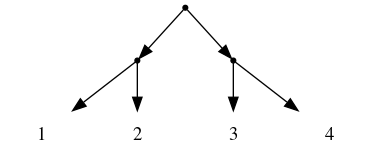
\includegraphics[width=\textwidth]{media/LeafTree.png}
\end{center}

While the type \texttt{BinTree} on \texttt{Int} represents trees such as
\begin{center}
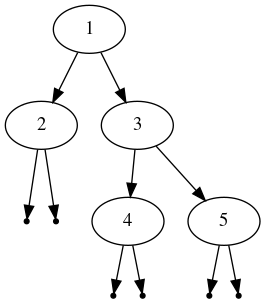
\includegraphics[width=\textwidth]{media/BinTree.png}
\end{center}

Also see \hyperref[sec:orga1ebb19]{More \texttt{LeafTree} and \texttt{BinTree} examples}.

\section*{Part 2: Flattening trees to lists          [20 points]}
\label{sec:org633ef12}
Implement a function named \texttt{flatten} for our two tree types
defined avoid, each of which convert the trees to lists,
discarding the tree structure.
Specifically,
\begin{enumerate}
\item the first \texttt{flatten} should have type \texttt{LeafTree[A] => List[A]}, and
\item the second \texttt{flatten} should have type \texttt{BinTree[A] => List[A]}.
\end{enumerate}

Note that we are able to reuse the name \texttt{flatten} for two different
functions so long as the type signatures are different.
\textbf{Edited September 18th}:
If this is not possible in your implementation of Scala,
name the two functions something similar instead, such as \texttt{flattenBT}.

For the \texttt{LeafTree} type, the elements should appear in the same
left-to-right order as they did in the tree.
So the above example tree would flatten to the list \texttt{[1,2,3,4]}.

For the \texttt{BinTree} type, for a given node \texttt{N},
all elements in the left subtree of \texttt{N}
should appear in the list \emph{before} the element of said node, and
all elements in the right subtree of that node
should appear in the list \emph{after} the element of said node.
So the above example tree would flatten to \texttt{[2,1,4,3,5]}.

\section*{Part 3: Elements of a \texttt{Tree[Int]} in order   [20 points]}
\label{sec:orgf0ddb63}
For each of the two tree types we have implemented, implement
a function \texttt{orderedElems} which converts trees containing integers
into lists \emph{which are sorted in \textbf{increasing} order}. So,
\begin{enumerate}
\item the first \texttt{orderedElems} should have type \texttt{LeafTree[Int] => List[Int]}, and
\item the second \texttt{orderedElems} should have type \texttt{BinTree[Int] => List[Int]}
\end{enumerate}
and in each case you must ensure the result is ordered
in increasing order.

\textbf{Edited September 18th}:
As in part 2, if your implementation of Scala does not support
giving these two functions the same name,
name them something similar instead.

You must implement your own sorting function on integer lists,
not use any builtin or library functions.

The marking of these functions will take into account
the \emph{elegance} of the solution.
\begin{center}
\textbf{Try to avoid unnecessary or repeated work.}
\end{center}

\textbf{Edited September 17th}: that said, based on statements I (Mark)
have made to inquiring students, and because this is the first homework,
the marking of this homework will still assign
at least a “good” mark to any solution
which matches the description in the first two paragraphs.

\section*{Part 4: Trees which describe structure     [10 points]}
\label{sec:orgeeac7c6}
Implement one additional type of unordered binary trees which,
given arbitrary types \texttt{A} and \texttt{B},
carry elements of \texttt{A} in their non-leaf nodes
and elements of \texttt{B} in their leaf nodes.
Call this type \texttt{StructTree}.
\begin{itemize}
\item This naming is inspired by the fact that these trees
can be seen as an \texttt{A} labelled structure
on top of elements of \texttt{B}.
Note the similarity to parse trees.
\end{itemize}

\textbf{Edited September 17th}: The correct way to write two type parameters
on a definition is \texttt{StructTree[A,B]}, not \texttt{StructTree[A][B]} as
I previously used below.

The type \texttt{StructTree[String,Int]} could be used
to represent trees such as
\begin{center}
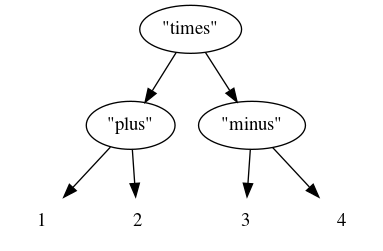
\includegraphics[width=\textwidth]{media/StructTree.png}
\end{center}

\section*{Part 5: Flattening structure trees   [bonus 20 points]}
\label{sec:orgf4be606}
Define an appropriate \texttt{flatten} operation for the \texttt{StructTree} type.

As this is a bonus question, there are many possible
interpretations of “appropriate”, and the marks for this question
will heavily depend upon which interpretation you use.

Try to come up with an implementation
which discards \emph{as little structure as possible},
bearing in mind that the transformation to lists
necessitates discarding at least some structure.
\section*{Testing}
\label{sec:org8315307}
\subsection*{Instructions}
\label{sec:orgcd2b7a7}
To test your solution, first complete
\href{./src/h1\_interface.sc}{this} interface script
by filling in the appropriate constructor/method invocations
in place of the \texttt{???}.
Save it in the same directory as your \texttt{h1.sc},
with the name \texttt{h1\_interface.sc}.

If you choose to complete the interface, you may also
choose to submit it along with your \texttt{h1.sc} file.

Then, save \href{./src/h1\_test.sc}{this} testing script
in the same directory, naming it \texttt{h1\_test.sc}, and invoke it with
\begin{minted}[breaklines=true]{shell}
amm h1_test.sc
\end{minted}

You do not need to submit the \texttt{h1\_test.sc} file.

If you are not using Ammonite, you will need to modify the tests
to work with your Scala implementation.
Simply placing their contents into your \texttt{h1.sc} file should work,
but be sure to remove them before submission.

\subsubsection*{Automated testing via Docker}
\label{sec:org54eb268}
You may use the \texttt{Dockerfile} and \texttt{docker-compose.yml} located at
\url{https://github.com/armkeh/principles-of-programming-languages/tree/master/homework/testing/h1}
to automate the system setup and testing.
Consult the \href{https://github.com/armkeh/principles-of-programming-languages/tree/master/homework/testing/h1/ReadMe.md}{README} located there for instructions.

The use of the shell scripts does require a \texttt{bash}-like shell.
On Windows, you may need to execute the commands in the shell scripts
manually instead.

\textbf{As the README states, you will need to copy your source files}
\textbf{to the \texttt{src} folder beneath the folder with the Docker setup}.
(Or, alternatively, use symbolic links to your source files.)

\subsection*{The scripts}
\label{sec:org03893f6}
The scripts are also shown here. First, the interface script.
\begin{minted}[breaklines=true]{scala}
import $file.h1, h1._
// Fill in your constructors here.

def BT_node[A](l: BinTree[A], a: A, r: BinTree[A]): BinTree[A] = ???
def BT_leaf[A]: BinTree[A] = ???
def BT_flatten[A](t: BinTree[A]): List[A] = ???
def BT_orderedElems(t: BinTree[Int]): List[Int] = ???

def LT_node[A](l : LeafTree[A], r: LeafTree[A]): LeafTree[A] = ???
def LT_leaf[A](a: A): LeafTree[A] = ???
def LT_flatten[A](t: LeafTree[A]): List[A] = ???
def LT_orderedElems(t: LeafTree[Int]): List[Int] = ???
\end{minted}

And the testing script.
\begin{minted}[breaklines=true]{scala}
import $file.h1_interface, h1_interface._

/* Given an expected result and a computed result,
   check if they are equal in value.
   If so, return 0. Otherwise, inform the user, and return 1,
   so the number of failures can be counted. */
def test[A](given: A, expected: A, the_test: String) =
  if (!(given equals expected)) {
    println("+---------------------------------------------------")
    println("| " + the_test + " failed.")
    println("| Expected " + expected + ", got " + given + ".")
    println("+---------------------------------------------------")
    1
  } else {
    0
  }



// Construct some simple trees of each type.
val bt_empty = BT_leaf
val bt_1 = BT_node(BT_leaf, 1, BT_leaf)
val bt_231 = BT_node(BT_node(BT_leaf, 2, BT_leaf), 3, BT_node(BT_leaf, 1, BT_leaf))

val lt_1 = LT_leaf(1)
val lt_231 = LT_node(LT_leaf(2), LT_node(LT_leaf(3), LT_leaf(1)))

// The tests are saved as tuples, the pieces of which will be passed
// to test.
val tests = List(
  (BT_flatten(bt_empty), List(), "Flattening an empty BinTree"),
  (BT_flatten(bt_1), List(1), "Flattening a BinTree singleton"),
  (BT_flatten(bt_231), List(2,3,1), "Flattening 2 / 3 \\ 1"),
  (BT_orderedElems(bt_231), List(1,2,3), "Ordering elements of 2 / 3 \\ 1"),
  (LT_flatten(lt_1), List(1), "Flattening a LeafTree singleton"),
  (LT_flatten(lt_231), List(2,3,1), "Flattening 2 /\\ (3 /\\ 1)"),
  (LT_orderedElems(lt_231), List(1,2,3), "Ordering elements of 2 /\\ (3 /\\ 1)"),
  )

// Apply test to each element of tests, and sum the return values.
// This is essentially a for loop.
val failed = tests.foldLeft(0) {
  (failures, next) => next match {
    // Deconstruct the tuple to get its parts
    case (given, expected, the_test) => failures + test(given, expected, the_test)
  }
}

println("+---------------------------------------------------")
println("| " + failed + " tests failed")
println("+---------------------------------------------------")
\end{minted}

\section*{More \texttt{LeafTree} and \texttt{BinTree} examples}
\label{sec:orga1ebb19}
Motivated by discussion of what is a proper \texttt{BinTree} or \texttt{LeafTree},
I have produced a few more examples here.

\subsection*{\texttt{LeafTree}}
\label{sec:orga5cb17a}
The \texttt{LeafTree} type still consists of binary trees.
Every (non-leaf) node must have two children,
and they are either non-leaf nodes or leaves.

Note that nothing says the tree must be balanced or ordered
in any way, as this example should hopefully convey.
\begin{center}
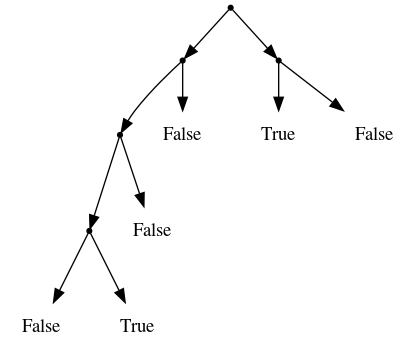
\includegraphics[width=\textwidth]{media/LeafTree2.png}
\end{center}

\subsection*{\texttt{BinTree}}
\label{sec:orgdbd9ddf}
It is possible to think of our \texttt{BinTree} type allowing each node
to have 0, 1 or 2 children.
But it is likely easier to represent and perhaps understand
if we think of every (non-leaf) having exactly two children,
with the possibility that one or both of them are the “empty tree”.

This example shows several nodes which seem to have one child only
in this way.
\begin{center}
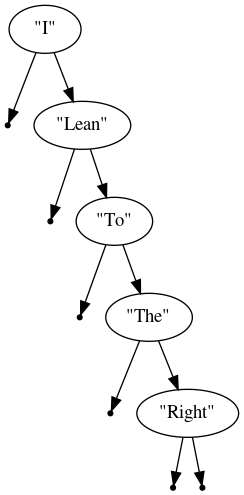
\includegraphics[width=\textwidth]{./media/BinTree2.png}
\end{center}
\end{document}
